\vspace{-0.5em}
\section{Introduction}
\label{sec:introduction}
\vspace{-0.5em}

%\begin{figure}
%  \centering
%  \begin{subfigure}[b]{0.25\textwidth}
%    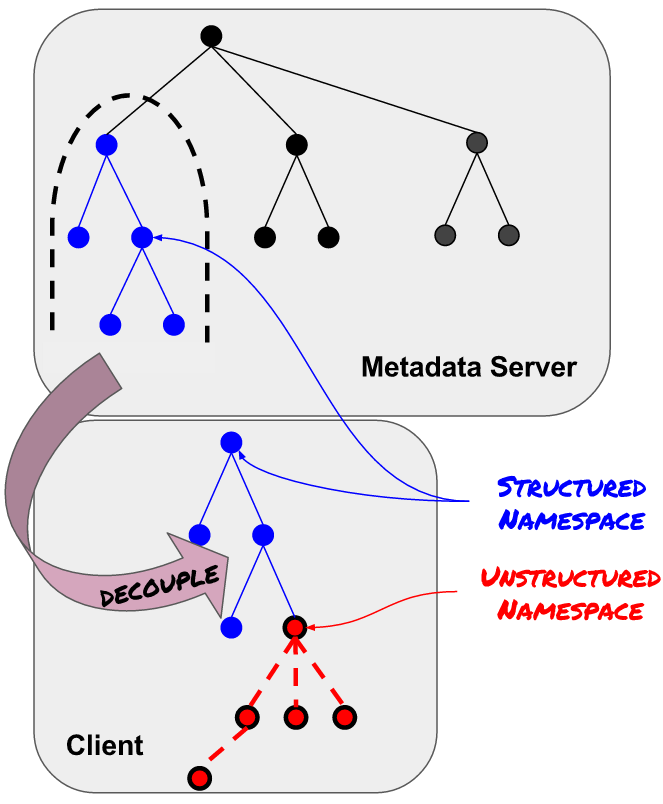
\includegraphics[width=\textwidth]{figures/intro.png}
%   \label{fig:intro}
%  \end{subfigure}
%  ~ 
%  \begin{subfigure}[b]{0.3\textwidth}
%    \begin{tabular}{ r | l }
%      Type         & Overhead       \\\hline\\
%      Structured   & 1 RPC          \\
%      Namespace    & O(1)           \\\\\hdashline\\
%      Unstructured & 1 RPC + Replay \\
%      Namespace    & O(1)           \\\\\hdashline\\
%      Traditional  & \(n\) RPCs     \\
%      Namespace    & O(\(n\))       \\
%    \end{tabular}
%    \\\\\\ % I am a hack
%   \label{table:intro}
%  \end{subfigure}
%  \caption{Clients decouple the file system subtrees and interact with their
%  private copiese locally for high performance. They can specify the structure of
%  the metadata they intend to create (structured namespace) or they can create
%  ad-hoc metadata (unstructured namespace), which is merged later.}
%\end{figure}
%    \caption{Traditional namespaces require at least 1 RPC per metadata
%    operation. Structured namespaces only need the initial RPC so clients/servers
%    understand (and can construct) the namespace.  Unstructured namespaces cannot
%    be parallelized and must replay metadata one by one onto the global namespace}

The file system metadata service is the scalability bottleneck for many of
today's workloads~\cite{roselli:atec2000-FS-workloads,
abad:techreport2012-fstrace, abad:ucc2012-mimesis,
alam:pdsw2011-metadata-scaling, weil:osdi2006-ceph}.  Common approaches for
attacking this ``metadata scaling wall" include: caching inodes on clients and
servers~\cite{depardon:tech13-survey, sinnamohideen:atc2010-ursa,
hildebrand:msst2005-pnfs, devulapalli:ipdps07-pvfs2, welch:fast2008-panasas},
caching parent inodes for path traversal~\cite{patil:fast2011-giga+,
ren:sc2014-indexfs, brandt:msst2003-lh, weil:sc2004-dyn-metadata,
ren:sc2014-indexfs}, and dynamic caching policies that exploit workload
locality~\cite{xing:sc2009-skyfs, zhu:pds2008-hba, li:msst2006-dynamic}.  These
caches reduce the number of remote procedure calls (RPCs) but the effectiveness
is dependent on the overhead of maintaining cache coherence and the
administrator's ability to select the best cache size for the given workloads.
Recent work reduces the number of metadata RPCs to 1 without using a cache at
all, by letting clients ``decouple" the subtrees from the global namespace so
that they can do metadata operations locally~\cite{zheng:pdsw2015-deltafs,
sevilla:ipdps18-cudele}. {\it Even with} this technique, we show that file
system metadata is still a bottleneck because namespaces for today's workloads
can be very large. The size is problematic for reads because metadata needs to
be transferred and materialized.

% What is our solution
The management techniques for file system metadata assume that namespaces have
no structure but we observe that this is not the case for all workloads. We
propose Tintenfisch, a file system that allows users to succinctly express the
structure of the metadata they intend to create.  If a user can express the
structure of the namespace, Tintenfisch clients and servers can (1) compact
metadata, (2) modify large namespaces more quickly, and (3) generate only
relevant parts of the namespace. This reduces network traffic, storage
footprints, and the number of overall metadata operations needed to complete a
job. 

Figure~\ref{fig:intro} provides an architectural overview: clients first
decouple the file system subtree they want to operate on\footnote{This is not a
contribution as it was presented in~\cite{sevilla:ipdps18-cudele}.} then
clients and metadata servers lazily generate subtrees as needed using a
``namespace generator". The namespace generator is stored in the root inode of
the decoupled subtree and can be used later to efficiently merge new metadata
(that was not explicitly stated up front) into the global namespace.  The
fundamental insight is that the client and server both understand the final
structure of the file system metadata. Our contributions:
\vspace{-0.5em}
\begin{itemize}
  \setlength\itemsep{-0.5em}

\item observing namespace structure in high performance computing, high energy
physics, and large fusion simulations (\S\ref{sec:motivating-examples})

\item based on these observations, we defined namespace schemas for
categorizing namespaces and their amenability to compaction and generation
(\S\ref{sec:namespace-schemas})

\item a generalization of existing file storage system services to implement
namespace generators that efficiently compact and generate metadata
(\S\ref{sec:namespace-generators})
\end{itemize}

\begin{figure}[t]
  \centering
  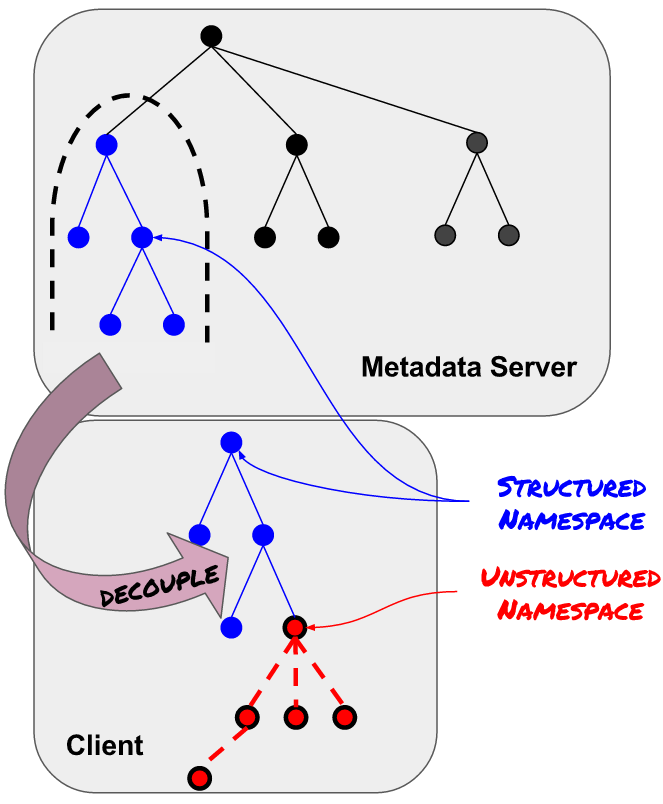
\includegraphics[width=0.8\linewidth]{figures/intro.png}
  \caption{In (1), clients decouple file system subtrees and interact with
their copies locally. In (2), clients and metadata servers generate subtrees,
reducing network/storage usage and the number of metadata operations.
\label{fig:intro}}
\end{figure}
